\documentclass[a4paper,11pt]{article}
% Préambule commun -- MOD08 Contrôles loi normale BTS MS, v1_0
\usepackage[utf8]{inputenc}
\usepackage[T1]{fontenc}
% babel-french absent sur certains postes : chargement conditionnel
\IfFileExists{french.ldf}{\usepackage[french]{babel}}{}
\usepackage{helvet}
\usepackage{courier}
\renewcommand{\familydefault}{\sfdefault}
\usepackage[top=3cm, bottom=2.5cm, left=2cm, right=2cm, headheight=2cm]{geometry}
\usepackage{amsmath,amssymb,amsfonts}
\usepackage{graphicx}
\usepackage[dvipsnames,table]{xcolor}
\usepackage{tikz}
\usepackage[most]{tcolorbox}
\usepackage{fancyhdr}
\usepackage{enumitem}
\usepackage{array,needspace,booktabs}
\usepackage{titlesec}
\usepackage{hyperref}

\definecolor{uimmblue}{HTML}{005C85}
\definecolor{uimmred}{HTML}{D31326}
\definecolor{uimmlightblue}{HTML}{E8F1F8}
\definecolor{uimmgray}{HTML}{333333}
\definecolor{uimmlightgray}{HTML}{F5F5F5}
\hypersetup{colorlinks=true, linkcolor=uimmblue, urlcolor=uimmblue}

\titleformat{\section}{\Large\bfseries\color{uimmblue}}{}{0pt}{}[\vspace{2pt}{\color{uimmblue}\titlerule[1.2pt]}]
\setlist[enumerate,1]{label={\color{uimmblue}\textbf{\arabic*.}}, leftmargin=*}
\setlist[enumerate,2]{label=\alph*), leftmargin=*}
\setlist[itemize,1]{label={\color{uimmblue}\textbullet}}

\newtcolorbox{exo}[1]{colback=white, colframe=uimmblue, fonttitle=\bfseries\color{white},
  coltitle=white, title={#1}, boxrule=1pt, arc=2pt,
  left=8pt, right=8pt, top=5pt, bottom=6pt, before skip=8pt, after skip=6pt}
\newtcolorbox{consigne}{colback=uimmlightgray, colframe=uimmgray, boxrule=0.8pt, arc=3pt,
  left=8pt, right=8pt, top=4pt, bottom=4pt}
\newtcolorbox{rappel}{colback=uimmlightblue, colframe=uimmblue, fonttitle=\bfseries\color{white},
  coltitle=white, title={Rappels de cours}, boxrule=1pt, arc=2pt,
  left=8pt, right=8pt, top=3pt, bottom=4pt, before skip=6pt, after skip=4pt, fontupper=\normalsize}
\newtcolorbox{correction}[1][]{%
  colback=green!5, colframe=green!50!black,
  fonttitle=\bfseries\color{white}, title={\textsf{Correction}~#1},
  coltitle=white, boxrule=1pt, arc=3pt,
  left=8pt, right=8pt, top=6pt, bottom=6pt, before skip=8pt, after skip=8pt, breakable}

\newcommand{\pts}[1]{\hfill\mbox{\color{uimmred}\small\textbf{(#1)}}}
% Zone de réponse lignée : #1 = nombre de lignes
\newcommand{\zone}[1]{\par\smallskip\noindent\begin{tikzpicture}
  \foreach \i in {1,...,#1}{\draw[uimmgray!30] (0,-0.78*\i) -- (\linewidth-1pt,-0.78*\i);}
  \end{tikzpicture}\par\smallskip}
\newcommand{\source}[1]{{\footnotesize\color{uimmgray}\textbf{Réf.}\enspace #1}\par\smallskip}
\newcommand{\piege}[1]{\par\smallskip{\footnotesize\color{uimmred!80!black}\textbf{Erreurs attendues~:} #1}}
\newcommand{\bareme}[1]{\par\smallskip{\footnotesize\color{uimmblue}\textbf{Barème~:} #1}}
\newcommand{\LN}{Cours MOD08 \textit{Loi normale}}
\newcommand{\EnTete}[3]{%
\pagestyle{fancy}\fancyhf{}\renewcommand{\headrulewidth}{0pt}
\fancyhead[L]{\raisebox{-0.5\height}{
\includegraphics[height=1.5cm]{logo_uimm_placeholder.jpg}}}
\fancyhead[C]{\begin{minipage}{7cm}\centering
  {\small\color{uimmblue}\textbf{Pôle Formation UIMM - CVDL}}\\
  {\footnotesize\color{uimmgray} BTS MS 1\textsuperscript{re} année\\ Mathématiques}\end{minipage}}
\fancyhead[R]{{\small\color{#3}\textbf{MOD08 -- #1}}}
\fancyfoot[C]{{\color{uimmblue}\rule{\textwidth}{1pt}}\\[2pt]
  {\footnotesize\color{uimmgray} Pôle Formation UIMM -- Centre-Val de Loire \hfill S. JAUBERT \hfill #2 -- \thepage}}}
\EnTete{Contrôle AB}{Sujet AB -- Contrôle 1 h}{uimmred}
\newcommand{\GRP}{A -- B}
% paramètres : \GRP (AB ou CD), \TITRE
\begin{document}

\begin{tcolorbox}[colback=uimmred, colframe=uimmred, sharp corners, boxrule=0pt,
  left=14pt, right=14pt, top=8pt, bottom=8pt]
{\color{white}\LARGE\bfseries Contrôle -- MOD08 \hfill Groupes \GRP}\\[3pt]
{\color{white}\large La loi normale en maintenance \hfill Durée~: 1 h}
\end{tcolorbox}

\vspace{2pt}
\noindent{\small\renewcommand{\arraystretch}{1.5}%
\begin{tabular}{@{}>{\bfseries\color{uimmblue}}l@{\hspace{6pt}}p{8.6cm}@{\hspace{10pt}}>{\bfseries\color{uimmblue}}l@{\hspace{6pt}}p{3.2cm}@{}}
Nom, prénom~: & \dotfill & Groupe~: & \dotfill \\
 & & Note~: & \dotfill\ / 20 \\
\end{tabular}}

\begin{consigne}\small
\textbf{Consignes.} Durée $1$ h. Calculatrice autorisée, aucun document. Répondre sur le sujet, dans les zones prévues.
\begin{itemize}[leftmargin=12pt, itemsep=0pt, topsep=2pt]
  \item Pour chaque probabilité~: écrire l'évènement avec la variable aléatoire, la \textbf{standardisation} $z$, \textbf{puis} le résultat arrondi à $10^{-4}$. Un résultat seul ne rapporte pas tous les points.
  \item Barème indicatif~: exercice 1 sur 4 points, exercice 2 sur 5, exercice 3 sur 5, exercice 4 sur 6. Les exercices vont du plus simple au plus exigeant.
\end{itemize}
\end{consigne}

\begin{rappel}
\textbf{Lire une loi normale $\mathcal{N}(\mu\,;\sigma)$.} La courbe en cloche est centrée sur la moyenne $\mu$~; $\sigma$ est l'\textbf{écart-type}. La probabilité est l'\textbf{aire} sous la courbe, l'aire totale vaut $1$. La courbe est symétrique par rapport à $\mu$~: $P(X \leq \mu - a) = P(X \geq \mu + a)$. Règle 68 -- 95 -- 99,7~:\\
$P(\mu-\sigma\leq X\leq\mu+\sigma)\approx 0{,}68$, \ $P(\mu-2\sigma\leq X\leq\mu+2\sigma)\approx 0{,}95$, \ $P(\mu-3\sigma\leq X\leq\mu+3\sigma)\approx 0{,}997$.

\smallskip
\textbf{Centrer et réduire.} Pour se ramener à la loi normale centrée réduite $\mathcal{N}(0\,;1)$, on \textbf{centre} (on retranche $\mu$) puis on \textbf{réduit} (on divise par $\sigma$)~:
\[
Z = \frac{X-\mu}{\sigma} \sim \mathcal{N}(0\,;1), \qquad P(X \leq x) = P(Z \leq z) \ \text{ avec } \ z = \frac{x-\mu}{\sigma}.
\]
Le nombre $z$ donne la position de $x$ en \textbf{nombre d'écarts-types} par rapport à la moyenne~: $z>0$ au-dessus de $\mu$, $z<0$ en dessous.

\begin{center}
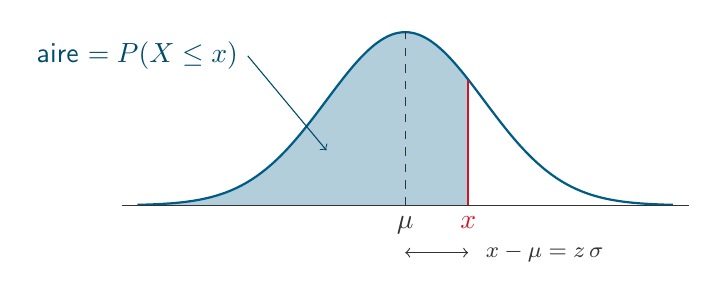
\begin{tikzpicture}[x=1cm,y=1cm]
  \fill[uimmblue!30, domain=-3.2:0.8, samples=60] (-3.2,0) -- plot (\x,{2.2*exp(-\x*\x/2)}) -- (0.8,0) -- cycle;
  \draw[uimmblue, thick, domain=-3.4:3.4, samples=80, smooth] plot (\x,{2.2*exp(-\x*\x/2)});
  \draw[uimmgray] (-3.6,0) -- (3.6,0);
  \draw[uimmgray, dashed] (0,0) -- (0,2.25);
  \draw[uimmred, thick] (0.8,0) -- (0.8,{2.2*exp(-0.32)});
  \node[below, uimmgray] at (0,-0.02) {$\mu$};
  \node[below, uimmred] at (0.8,-0.02) {$x$};
  \node[uimmblue!80!black, anchor=east] at (-2.0,1.9) {aire $= P(X \leq x)$};\draw[->, uimmblue!80!black] (-2.0,1.9) -- (-1.0,0.7);
  \draw[<->, uimmgray] (0,-0.6) -- (0.8,-0.6);
  \node[right, uimmgray, font=\footnotesize] at (0.9,-0.6) {$x - \mu = z\,\sigma$};
\end{tikzpicture}
\end{center}
\textbf{Calculer une probabilité.} $P(X > a) = 1 - P(X \leq a)$~; \ $P(a \leq X \leq b) = P(X \leq b) - P(X \leq a)$~; \ $P(X = a) = 0$.

\smallskip
\textbf{Problème inverse (chercher un seuil).} On cherche $x$ tel que $P(X \leq x) = p$ (aire \textbf{à gauche} de $x$). On lit $z$ sur la loi centrée réduite, puis $x = \mu + z\,\sigma$. Si l'énoncé donne une aire à droite, on passe à l'aire à gauche~: $P(X > x) = q \iff P(X \leq x) = 1-q$. Pour chercher $\mu$ ou $\sigma$, on garde le même $z$~: $\mu = x - z\,\sigma$ \ ou \ $\sigma = \dfrac{x-\mu}{z}$.\\
\textbf{Arrondi}~: on arrondit dans le sens qui \textbf{respecte l'exigence} de l'énoncé, pas forcément au plus proche.

\smallskip
\textbf{Calculatrice.} Probabilité~: TI \texttt{normalFRép(a,b,$\mu$,$\sigma$)}, Casio \texttt{Ncd} (borne infinie~: \texttt{-1E99} ou \texttt{1E99}). Seuil~: TI \texttt{FracNormale($p$,$\mu$,$\sigma$)}, Casio \texttt{InvN} (aire à gauche~; Casio~: saisir $\sigma$ avant $\mu$).
\end{rappel}

\newpage


\section{Exercice 1 -- Température d'un palier de pompe \hfill {\normalsize\color{uimmred}4 points}}
\begin{exo}{Alarme de température}
Sur une pompe d'alimentation, un capteur mesure la température $T$ (en $^\circ$C) du palier côté accouplement. En fonctionnement normal, $T$ suit la loi normale d'espérance $\mu = 62$ et d'écart-type $\sigma = 4$. Une alarme se déclenche dès que $T$ dépasse $70\,^\circ$C.
\end{exo}
\begin{enumerate}
  \needspace{5.0cm}
  \item Calculer le nombre $z$ associé à $70\,^\circ$C. Dire en une phrase ce que représente ce nombre. \pts{1 pt}
  \zone{4}
  \needspace{5.8cm}
  \item Calculer $P(T > 70)$. Combien d'alarmes intempestives attend-on, en moyenne, sur $1\,000$ relevés en fonctionnement normal~? \pts{1 pt}
  \zone{5}
  \needspace{5.8cm}
  \item Calculer $P(58 \leq T \leq 66)$. Comparer avec la règle 68 -- 95 -- 99,7. \pts{1 pt}
  \zone{5}
  \needspace{5.8cm}
  \item Une température inférieure à $55\,^\circ$C signale une pompe qui tourne presque à vide. Calculer la probabilité d'un tel relevé en fonctionnement normal. \pts{1 pt}
  \zone{5}
\end{enumerate}

\newpage
\section{Exercice 2 -- Courroies de convoyeurs \hfill {\normalsize\color{uimmred}5 points}}
\begin{exo}{Remplacement préventif}
Une usine exploite $80$ convoyeurs à courroie identiques. La durée de fonctionnement $D$ (en heures) d'une courroie avant rupture suit la loi normale d'espérance $\mu = 12\,000$ et d'écart-type $\sigma = 1\,500$. Le service maintenance remplace chaque courroie, par précaution, à $9\,000$ h de fonctionnement.
\end{exo}
\begin{enumerate}
  \needspace{5.8cm}
  \item Calculer la probabilité qu'une courroie casse \textbf{avant} son remplacement préventif. \pts{1 pt}
  \zone{5}
  \needspace{5.0cm}
  \item En moyenne, combien de courroies sur les $80$ casseront avant leur remplacement~? \pts{1 pt}
  \zone{4}
  \needspace{5.8cm}
  \item Calculer la probabilité qu'une courroie dure entre $9\,000$ h et $14\,000$ h. \pts{1,5 pt}
  \zone{5}
  \needspace{5.8cm}
  \item Sans nouveau calcul à la calculatrice, déduire $P(D > 15\,000)$ de la question 1, en justifiant par la symétrie de la courbe. \pts{1,5 pt}
  \zone{5}
\end{enumerate}

\newpage
\section{Exercice 3 -- Revoir la date de remplacement \hfill {\normalsize\color{uimmred}5 points}}
\begin{exo}{Mêmes courroies, nouvelle exigence}
Les courroies de l'exercice 2 ($D$ suit $\mathcal{N}(12\,000\,;1\,500)$) sont conservées. Le responsable trouve trop élevée la proportion de casses avant remplacement. Il exige désormais que \textbf{au plus $1\,\%$} des courroies cassent avant la date de remplacement $t$ (en heures).
\end{exo}
\begin{enumerate}
  \needspace{5.8cm}
  \item Écrire l'exigence sous la forme $P(D < t) \leq 0{,}01$. Chercher le nombre $z$ tel que $P(Z < z) = 0{,}01$ (loi centrée réduite). \pts{1 pt}
  \zone{5}
  \needspace{7.4cm}
  \item En déduire la plus grande date $t$, \textbf{en heures entières}, qui respecte l'exigence. Justifier le sens de l'arrondi. \pts{2 pts}
  \zone{7}
  \needspace{6.6cm}
  \item Le service méthodes veut étudier les $20\,\%$ de courroies les plus durables. À partir de quelle durée $x$ (arrondie à l'heure) une courroie fait-elle partie de ce groupe~? \pts{2 pts}
  \zone{6}
\end{enumerate}

\newpage
\section{Exercice 4 -- Pression du réseau d'air comprimé \hfill {\normalsize\color{uimmred}6 points}}
\begin{exo}{Arrêts de machines pneumatiques}
Dans un atelier, la pression $X$ (en bar) du réseau d'air comprimé suit la loi normale d'espérance $\mu = 6{,}4$ et d'écart-type $\sigma = 0{,}25$. Les machines pneumatiques s'arrêtent dès que $X$ est inférieure à $6{,}0$ bar. Le cahier des charges exige $P(X < 6{,}0) \leq 0{,}005$.
\end{exo}
\begin{enumerate}
  \needspace{5.0cm}
  \item Calculer $P(X < 6{,}0)$. \pts{1,5 pt}
  \zone{4}
  \needspace{4.2cm}
  \item Le cahier des charges est-il respecté~? Justifier. \pts{1 pt}
  \zone{3}
  \needspace{6.6cm}
  \item L'écart-type reste égal à $0{,}25$ et on règle la pression moyenne $\mu$. Quelle est la plus petite valeur de $\mu$, \textbf{au centième de bar}, qui respecte le cahier des charges~? Justifier l'arrondi. \pts{2 pts}
  \zone{6}
  \needspace{6.6cm}
  \item La moyenne reste égale à $6{,}4$ et on améliore la régulation pour réduire $\sigma$. Quelle est la plus grande valeur de $\sigma$, \textbf{au centième de bar}, qui respecte le cahier des charges~? \pts{1,5 pt}
  \zone{6}
\end{enumerate}
\end{document}
